\documentclass[
a4paper, 12pt, % Papierformat, Schriftgröße
titlepage, 		 % extra Titelseite statt einfacher Überschrift
twoside,			 % beidseitiger Druck
headsepline,	 % Trennlinie für die Kopfzeile
BCOR5mm,			 % Binderand 5 mm
idxtotoc, bibtotoc]{scrreprt}	% Index (soweit vorhanden) und Literaturliste 
				       % im Inhaltsverzeichnis aufführen
% Dokumentenklasse ist aus dem KOMA-Script-Paket die SCRReprt-Klasse.

\usepackage{wsi-ra}

%%%%%%%%%%%%%%%%%%%%%%%%%%%%%%%%%
% Gestaltung der Titelseite     %
%%%%%%%%%%%%%%%%%%%%%%%%%%%%%%%%%

\titlehead{\vspace{.5cm}\centering
\textbf{\textsc{Eberhard-Karls-Universität Tübingen}}\\
Wilhelm-Schickard-Institut für Informatik\\Lehrstuhl Rechnerarchitektur}

\subject{\large Diplomarbeit}
% Studien-, Bachelor-, Diplom- oder Masterarbeit

% Der Titel
\title{\begin{tabular}{p{11cm}}\centering\Large
Das Format von Abschlussarbeiten am Lehrstuhl Rechnerarchitektur
\end{tabular}}


% Der Name des Autors
\author{\large Max Mustermann}
\date{} % Hier kein Datum eintragen!

% Die Betreuer sowie das Abgabedatum etc.
\publishers{\normalsize\centering\begin{tabular}{p{3cm}p{8cm}}
\textbf{Betreuer:} 	& Prof.\,Dr.\,rer.\,nat.~Andreas Zell\\
			& Wilhelm-Schickard-Institut für Informatik\\
      & \\
			& Prof.\,Dr.\,rer.\,nat.~Zweitbetreuer\\
			& Institut für interessante Biologie\\
      & \\
\textbf{Begonnen am:}	& \\
 			& \\
\textbf{Beendet am:}	& \today
\end{tabular}}


%%%%%%%%%%%%%%%%%%%%%%%%%%%%%%%%%
% Eidesstattliche Erklärung     %
%%%%%%%%%%%%%%%%%%%%%%%%%%%%%%%%%

\uppertitleback{\ \\[4ex]\centering
\begin{tabular}{>{\normalsize}p{4.5cm}>{\normalsize}p{4cm}}
\large\textbf{Erklärung} & \\[4ex] \multicolumn{2}{p{8.5cm}}{\normalsize
Hiermit versichere ich, diese Arbeit selbstständig verfasst und nur die
angegebenen Quellen benutzt zu haben.}\\
\\[2ex]\multicolumn{2}{p{8.5cm}}{\normalsize Tübingen am \today}\\[6ex]
\begin{tabular}{p{4.2cm}}\cline{1-1}\\\end{tabular}&\\
Max Mustermann
\end{tabular}}
\lowertitleback{} % Hier nichts eintragen!


%%%%%%%%%%%%%%%%%%%%%%%%%%%%%%%%%
% Beginn des Dokumentes         %
%%%%%%%%%%%%%%%%%%%%%%%%%%%%%%%%%

\begin{document}


%%%%%%%%%%%%%%%%%%%%%%%%%%%%%%%%%
% Titelei                       %
%%%%%%%%%%%%%%%%%%%%%%%%%%%%%%%%%

\pagenumbering{roman}		% kleine lateinische Seitenzahlen
\maketitle

\begin{abstract}
\textbf{Kurzfassung. }Dieses Dokument soll zeigen, wie mit \LaTeXe{} eine Abschlussarbeit entsprechend
der Richtlinien am Lehrstuhl Rechnerarchitektur erstellt werden kann. Es handelt
sich hierbei weder um eine Einführung in \LaTeX, noch in wissenschaftliche
Methode oder Schreibweise. Es werden einige Stilelemente und häufige
Schwierigkeiten exemplarisch herausgegriffen und vorgestellt. Ferner soll kurz
Aufbau und Benutzung dieser Vorlage beschrieben werden. Weiterführende Literatur
ist im Anhang aufgeführt. Zu den hier dargestellten \LaTeX-Paketen existieren
weiterhin eigene Dokumentationen, die nicht alle im Literaturverzeichnis
aufgeführt sind. Diese Vorlage basiert auf dem \KOMAScript-Paket
\cite{Neukam2003}, da hier die Dokumentenklasse Report (\verb!scrreprt!)
verwendet wird. Wichtig ist, dass die getätigten Einstellungen in diesem
Dokument nicht verändert werden, außer wenn statt in deutscher lieber in
englischer Sprache geschrieben wird. Dazu sind bereits einige Pakete vorgesehen,
die aber z.\,T. mit Kommentaren versehen und somit nicht aktiv sind. Die Datei
\verb!Vorlage.tex! dient als Hauptdokument. Der eigentliche Text sollte aber in
einer eigenen Datei pro Kapitel geschrieben werden, die dann lediglich in das
Hauptdokument eingebunden werden müssen. Dieses Vorgehen wird mit einem Kapitel
beispielhaft dargestellt. Ebenso können vorhandene Quelltexte direkt in das
Dokument integriert oder als Pseudocode aufgelistet werden. Auch wird
beispielhaft die Verwendung von Unterabbildungen, langen und normalen Tabellen
sowie mathematischen Formeln gezeigt. Abschließend wird kurz auf weiterführende
Literatur eingegangen. Ebenso beispielhaft werden im Abkürzungsverzeichnis
einige Einträge vorgenommen. Generell sollen nur verwendete Abkürzungen, die
nicht im Duden enthalten sind, in dieses Verzeichnis aufgenommen werden.
\end{abstract}

\chapter*{Danksagung}
Ich danke allen, die an dieser Arbeit mitgewirkt haben. Eine Danksagung ist
grundsätzlich nicht nötig und darf durchaus entfallen. Falls gewünscht, ist die
Danksagung an dieser Stelle einzufügen.


\tableofcontents		% Inhaltsverzeichnis
\cleardoublepage		% Erzeugt neue Leerseite. Muss ggf. auskommentiert werden.
\pagenumbering{arabic}		% Ab hier mit arabischen Zahlen numerieren


%%%%%%%%%%%%%%%%%%%%%%%%%%%%%%%%%
% Beginn der eigentlichen Arbeit%
%%%%%%%%%%%%%%%%%%%%%%%%%%%%%%%%%

\chapter{Einführung}

\section{Aller Anfang ist schwer}

Immer wieder treten Probleme bei der Erstellung von Abschlussarbeiten auf.
Dieses Dokument soll nun exemplarisch darlegen, wie am Lehrstuhl
Rechnerarchitektur alle Abschlussarbeiten -- sowohl Studien-, Bachelor-, Diplom-
als auch Masterarbeiten -- angefertigt werden. Der Stil wird durch dieses
Dokument festgelegt. Ebenso sind in dieser Vorlage bereits zahlreiche Pakete
eingebunden, die i.\,d.\,R. für eine solche Arbeit ausreichen sollten. In
manchen Fällen könnten zusätzliche Pakete notwendig werden. Vor deren Einbindung
ist allerdings zu prüfen, ob sich das Paket eventuell schon in der Stildatei
\texttt{wsi-ra.sty} befindet. Gegebenenfalls ist der Betreuer darauf
anzusprechen.

Prinzipiell gibt dieses Dokument auch einen Vorschlag für die Gliederung einer
Abschlussarbeit:
\begin{enumerate}
\item Einführung
\item Material und Methoden
\item Ergebnisse
\item Diskussion
\item Schlussfolgerungen [sofern nicht schon im Kapitel Diskussion]
\item Zusammenfassung [und ggf. Ausblick]
\end{enumerate}
Daran schließt sich der Anhang an, der normalerweise nur aus dem Literatur- und
Abkürzungsverzeichnis\footnote{Die Benutzung des Abkürzungsverzeichnisses ist
der Dokumentation zum zu Grunde liegenden Paket \texttt{juraabbrev} zu
entnehmen} besteht. In einigen Fällen könnte ein Glossar oder ein Index
erforderlich werden. Dafür sind bereits notwendige Pakete und Einstellungen
vorgesehen. Bei Bedarf muss lediglich das Paket \texttt{makeidx} benutzt
werden. Um Glossareinträge zu schreiben, kann sich an den (auskommentierten)
Beispieleinträgen orientiert werden, die sich in der Glossardatei im
\texttt{tex}-Verzeichnis befinden. Damit die Einträge darin automatisch
sortiert werden, ist folgender Aufruf auf der Kommandozeile (Linux) nötig:
\begin{verbatim}
makeindex -t Vorlage.glg -o Vorlage.gls -s \
  Vorlage.ist Vorlage.glo
\end{verbatim}
Hierbei steht der \emph{Backslash} übrigens für einen Zeilenumbruch innerhalb
eines Befehls und kann daher entfallen. Anschließend erst kann das Dokument mit
(PDF-) \LaTeX{} kompiliert werden. Wird kein Glossar verwendet, ist dieser
Aufruf auch nicht nötig.

Im Quelltext ist auch schon vorgesehen, dass die einzelnen Abschnitte durch eine
jeweils eigene Datei eingebunden werden. Dazu brauchen lediglich die Kommentare
entfernt und die Dateien angelegt werden sofern noch nicht vorhanden. Alle
\LaTeX-Dokumente liegen im Unterverzeichnis \texttt{tex}.

Weitere Verzeichnisse wie Tabellen-, Abbildungs- oder gar Algorithmenverzeichnis
sind nicht er\-wünscht und daher zu unterlassen. Die Seiteneinstellungen, die
Schriftart und -größe sind nicht zu verändern.

Der \verb!\cleardoublepage!-Befehl vor Beginn der Einführung ist notwendig, um
zu verhindern, dass eine rechte Seite eine Seitenzahl auf der Innenseite erhält.
Sollte Das Inhaltsverzeichnis länger als eine Seite sein, ist diese Anweisung zu
entfernen. Dieser Befehl ist ggf. auch dann zu entfernen, wenn keine Danksagung
erfolgt. Für Danksagungen ist zu beachten, dass durch diese der Eindruck
entstehen könnte, die Arbeit sei nicht selbstständig angefertigt worden. Daher
sind diese entweder ganz zu unterlassen, oder äußerst kurz zu fassen.
Widmungen sind nicht erwünscht.


\section{Umfang von Abschlussarbeiten}

Am Lehrstuhl Rechnerarchitektur haben Bachelorarbeiten einen Umfang von 40 bis
60 Seiten. Die Obergrenze ist durch die PSO Informatik und Bioinformatik
vorgegeben, die Untergrenze durch Prof.~Zell. Studienarbeiten haben einen Umfang
von 40 bis 60 Seiten, wobei dort die Obergrenze nicht hart ist. In jedem Fall
soll die Länge unter 70 Seiten bleiben, was der alten Vorgabe entspricht.
Optimal sind bei beiden Arbeiten 50 Seiten inclusive aller Abbildungen,
Literaturangaben und der Titelei.

Masterarbeiten haben einen Umfang von 50 bis 99 Seiten, wobei die Ordnungen nur
den zeitlichen Umfang auf sechs Monate limitieren. Gleiches gilt für
Diplomarbeiten am Lehrstuhl Rechnerarchitektur. Optimal sind bei beiden Arbeiten
70 Seiten.

Die Schrift- und Randgröße spielt für den Umfang, also die Seitenzahl eine große
Rolle. Daher sollen diese Einstellungen in dieser Vorlage keinesfalls geändert
werden. Es sei jedoch darauf hingewiesen, dass die Bewertung der Arbeit keine
direkte Funktion der Seitenzahl ist.


\section{Druck und der Abgabe der fertigen Arbeit}

Grundsätzlich sollen alle Arbeiten doppelseitig auf DIN-A4-Papier gedruckt und
mit den im Sekretariat des Lehrstuhls Rechnerarchitektur erhältlichen grünen
Einbanddeckeln und der dafür vorgesehenen schwarzen Klebebindung (keine
Spiralbindung) gebunden werden.

Im Fall von Studien- und Bachelorarbeiten sind zwei Exemplare bei Prof.~Zell und
ein Exemplar beim jeweiligen Betreuer abzugeben. Weiterhin müssen zwei Exemplare
im Prüfungssekretariat abgegeben werden. Davon wird eines in die WSI-Bibliothek
und das zweite in das Archiv des Prüfungsamtes eingefügt.

Bei Diplom- und Masterarbeiten müssen ebenfalls zwei Exemplare bei Prof.~Zell,
zwei Exemplare im Prüfungssekretariat, mindestens ein Exemplar beim
Zweitkorrektor sowie ein Exemplar beim jeweiligen Betreuer abgegeben werden.


\section{Umstellung der Vorlage für englischsprachige Abschlussarbeiten}

Diese Vorlage geht davon aus, dass die Abschlussarbeit in deutscher Sprache
verfasst werden soll. Falls die Arbeit stattdessen in Englisch geschrieben
werden soll, müssen einige Umstellungen aus der Vorlage wieder rückgängig
gemacht werden. Diese Änderungen betreffen die Stildatei \texttt{wsi-ra.sty}
\begin{description}
 \item[Silbentrennung] Das Paket \verb!ngerman! muss auskommentiert, der
 Kommentar vor dem \verb!babel!-Paket jedoch entfernt werden. Als Option wird
 die Sprache übergeben:
 \begin{verbatim}
 \usepackage[english]{babel}
 \end{verbatim}
 Gegebenenfalls kann zusätzlich auch \verb!ngerman!
 in die eckige Klammer hinzugefügt werden (Sprachen durch Kommata getrennt).
 \item[Literaturverzeichnis] Statt \verb!\bibliographystyle{ra-alpha}! wird nun
 der Stil \verb!alpha! erforderlich. Der Präfix \verb!ra-! muss also entfernt
 werden. Das Paket \verb!bibgerm! wird dadurch überflüssig und kann
 auskommentiert werden.
 \item[Spracheinstellungen] Die im Hauptdokument unter dem Kommentar
 "`Einstellungen"' getroffenen Sprachdefinitionen zum Algorithmus-Paket, Glossar
 (soweit das Paket \verb!glossary! überhaupt eingebunden wurde) sowie zu
 Definitionen, Theoremen, Sätzen und Beweisen sind hinfällig und müssen
 auskommentiert bzw. angepasst werden. Des Weiteren muss an dieser
 Stelle für das Abkürzungsverzeichnis noch die folgende Zeile hinzugefügt
 werden:
 \begin{verbatim}
 \renewcommand{\abbrevname}{List of Abbreviations}
 \end{verbatim}
 \item[Glossar] Zur Verwendung eines Glossars in deutschsprachigen Dokumenten
  wurden unter "`Einstellungen"' folgende Befehle eingesetzt, die im Falle einer
  englischsprachigen Abschlussarbeit auskommentiert werden müssen:
  \begin{verbatim}
  \renewcommand{\glossaryname}{Glossar}
  \renewcommand{\descriptionname}{Beschreibung}
  \end{verbatim}
\end{description}


\section{Nützliche Programme zum Erstellen der Abschlussarbeit}

Auch \LaTeX{} muss heute nicht mehr komplett manuell in einen archaischen Editor
eingetippt werden. Es gibt inzwischen eine Reihe hilfreicher Programme, um die
Arbeit zu erleichtern. Einige davon seien im Folgenden genannt. Es kann hier
jedoch keine Vollständige Liste präsentiert werden.
Für Linux bieten sich an:
\begin{itemize}
 \item TeXstudio, \url{http://texstudio.sourceforge.net/}
 \item Kile, \url{http://kile.sourceforge.net}
 \item Lyx, \url{http://www.lyx.org}
\end{itemize}
Unter Windows stehen folgende Programme zur Verfügung:
\begin{itemize}
 \item TeXstudio, \url{http://texstudio.sourceforge.net/}
 \item {\TeX}niccenter, \url{http://www.texniccenter.org}
 \item Lyx, \url{http://wiki.lyx.org/Windows/Windows}
\end{itemize}
Nach Installation von KDE für Windows kann auch das Programm Kile unter Windows
genutzt werden. Im Abschnitt~\ref{sec:HinweiseLiteratur} auf Seite
\ref{sec:HinweiseLiteratur} wird weiterhin auf den nützlichen Referenzmanager
\textsc{JabRef} hingewiesen (Abbildung~\ref{fig:JabRef}, Seite
\ref{fig:JabRef}). Unter KDE kann als Alternative auch kbibtex benutzt werden.


\section{Wichtige Einstellungen beim Verwenden dieser Vorlage}

Es müssen unbedingt folgende Angaben verändert werden, bevor diese Vorlage
benutzt werden kann:
\begin{description}
 \item[subject] Statt "`Diplomarbeit"' muss hier einer der zulässigen
 Typen Studien-, Bachelor-, Diplom- oder Masterarbeit eingetragen werden.
 \item[title] Die \verb!tabular!-Anweisung darf nicht verändert werden. Dort
 wo der Beispieltitel steht, muss der eigene eingetragen werden.
 \item[author] Eigener Name! Dieser muss auch in der darauffolgenden
 eidesstattlichen Erklärung noch einmal von "`Max Mustermann"' auf den eigenen
 geändert werden.
 \item[Betreuer] Die beispielhaft angegebenen Betreuer müssen geändert werden.
 \item[Begonnen am] Hier muss das Datum eingetragen werden. Das Abgabedatum wird
 automatisch auf den aktuellen Tag gesetzt.
\end{description}
Um die Funktionalität von PDF\LaTeX{} nutzen zu können, sind ferner die
folgenden Felder interessant, die es erlauben Informationen über die Arbeit in
der PDF-Datei abzuspeichern. Diese können dann unter Dokumenteneigenschaften im
Acrobat Reader eingesehen und von Desktopsuchprogrammen indiziert werden.
\begin{description}
 \item[pdftitle] Der Titel der Arbeit. Dieser wird auch im Acrobat Reader in
der Titelleiste angezeigt.
 \item[pdfauthor] Hier soll nochmals der eigene Name eingetragen werden.
 \item[pdfsubject] Voreingetragen ist "`Abschulussarbeit"'. Dieser Eintrag
sollte durch den Typ der Arbeit ersezt werden (z.\,B. "'Diplomarbeit"' oder
"`Masterarbeit"').
 \item[pdfkeywords] Hier können durch Kommata separiert Stichworte eingetragen
werden, die den Inhalt der Arbeit charakterisieren. Typischer Weise sollten
diese erst gegen Ende der Arbeit festgelegt werden.
\end{description}
Zu finden sind diese Felder unter "`PDF\LaTeX- bzw. \LaTeX-spezifische
Einstellungen"'.


\section{Warnmeldungen beim Kompilieren}

Wenn diese Vorlage kompiliert wird, erscheinen ggf. mehrere Warnmeldungen --
abgesehen von Meldungen über \textit{under-} bzw. \textit{overfull hbox}.
Einige können umgangen werden, indem die betroffenen Stildateien (\texttt{mhchem},
\texttt{algorithm[ic]} und \texttt{abbrev}) in das \LaTeX-Verzeichnis jeweils
in ein eigenes Unterverzeichnis kopiert werden. Anschließende Ausführung des
\verb!texhash!-Kommandos behebt dann die Warnungen. Dieses Vorgehen ist aber
nicht unbeding notwendig, wenn z.\,B. nur einmalig eine Abschlussarbeit erstellt
werden soll, da sich die Vorlage dennoch kompilieren lässt.

\section{Fehler beim Kompilieren wegen des Abkürzungsverzeichnisses}

Pdflatex macht Probleme beim Kompilieren der Vorlage, da das abbrev-Skript abbricht, wenn die temporäre .abb-Datei bereits vorhanden ist. Wenn die .abb-Datei vor dem Aufruf von pdflatex gelöscht wird, funktioniert es dagegen einwandfrei. In TeXstudio kann man sich dafür eine eigene Regel erstellen. Dazu trägt man unter dem Menüpunkt (Options $\Rightarrow$ Configure TeXstudio $\Rightarrow$ Build $\Rightarrow$ User Commands) folgenden Befehl ein:

\begin{verbatim}
rm %.abb | pdflatex -synctex=1 -interaction=nonstopmode %.tex
| txs:///view-pdf-internal
\end{verbatim}

Wie man sieht besteht der Befehl aus drei Teilen: Löschen der .abb-Datei, Übersetzen mit pdflatex und Darstellen des resultierenden PDF-Dokuments mit dem Internen Betrachter.

Anschließend kann man diesen Befehl über den Menüpunkt (Tools $\Rightarrow$ User) oder über die dort angezeigte Tastenkombination starten.

\section{Beispiele für einige Stilelemente}
Falls sehr große Abbildungen oder Tabellen eingebunden werden sollen,
kann wahlweise eines der Pakete \verb!pdflscape! bzw. \verb!lscape! verwendet
werden, um auf Querformat umzuschalten. Beide Pakete sind vorgesehen. Da die
Pakete die Benutzung von \verb!pdflatex! bzw. \verb!latex! vorschreiben, wird
vor deren Einbindung überprüft, mit welchem Programm die Arbeit übersetzt wird.
Überschriften können trotzdem wie bei Hochkantformat gesetzt werden (siehe dazu
Internetquellen).

\subsection{Abbildungen}
Für normale Abbildungen ist es i.\,d.\,R. ausreichend, jeweils zwei
nebeneinander zu setzen. Dazu dient das Paket \verb!subfigure!. Ein Beispiel für
eine Abbildung mit zwei Unterabbildungen zeigt Abbildung~\ref{fig:ZweiBilder}.
\begin{figure}[htbp]
\centerline{
\subfigure[Titel dieses Bildes]{%
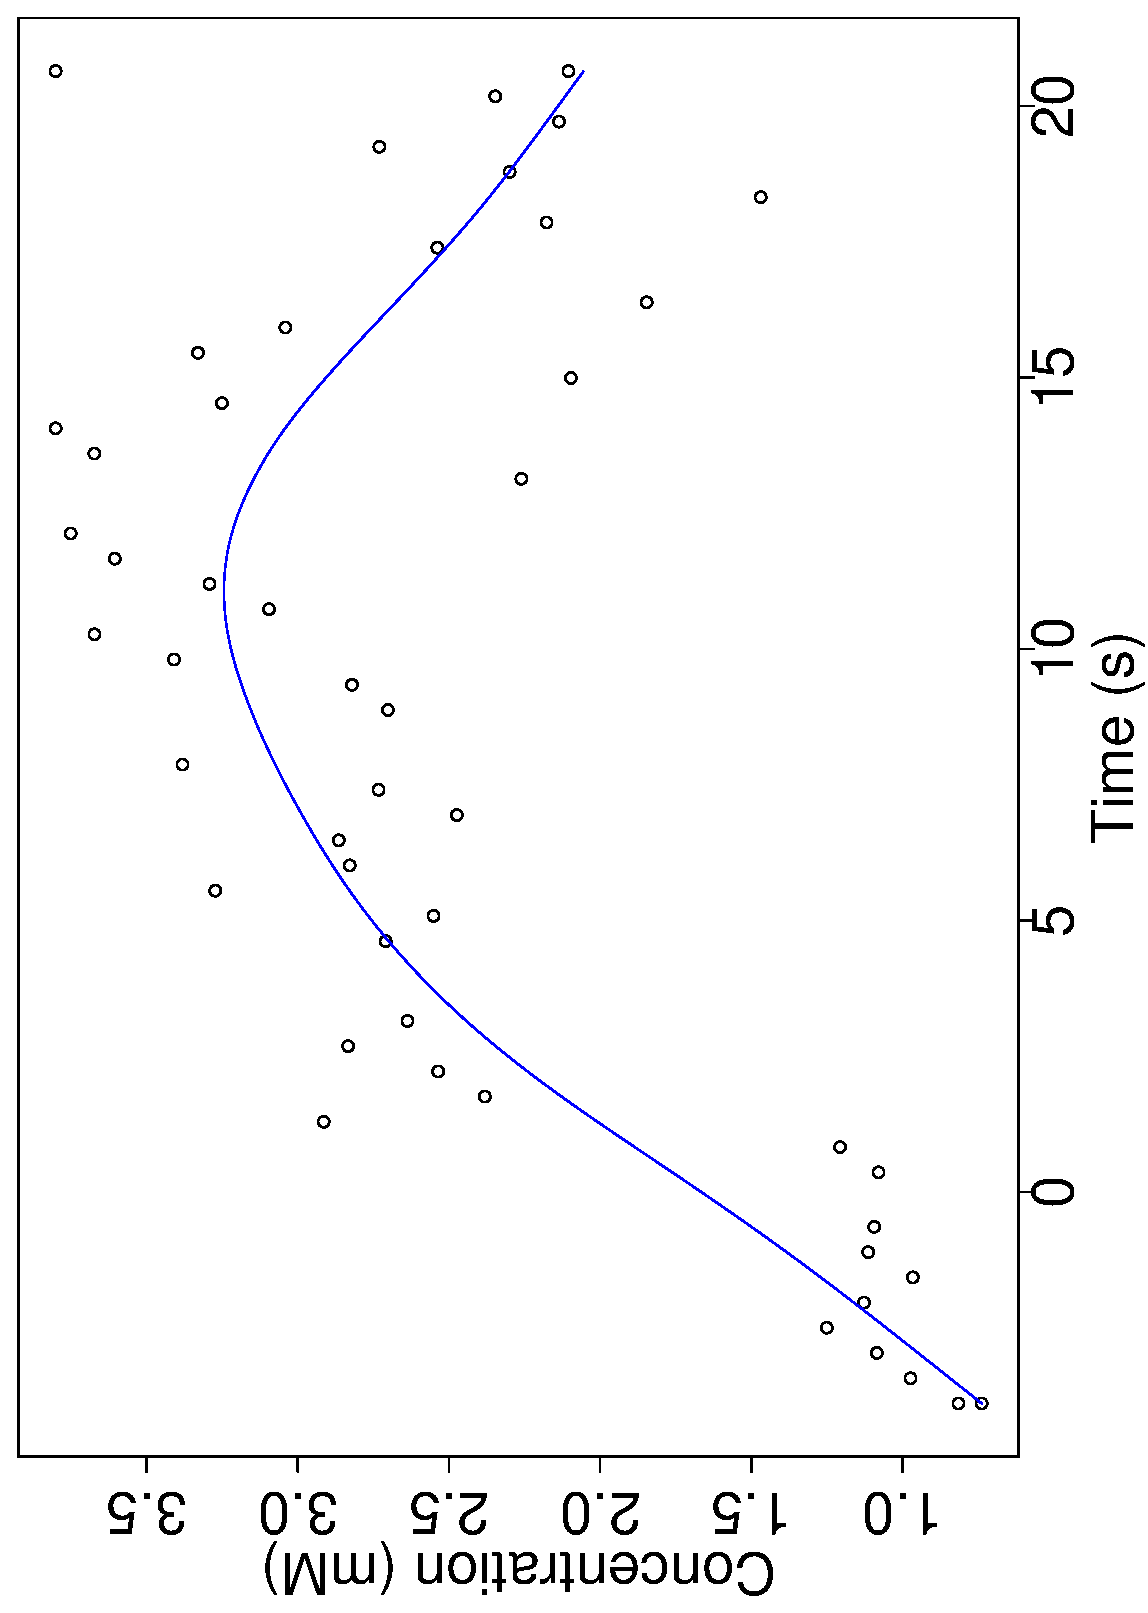
\includegraphics[width=.35\textwidth, angle=90]{img/plotAla}
\label{subfig:ErstesBild}}\hfill
\subfigure[Titel dieses Bildes]{%
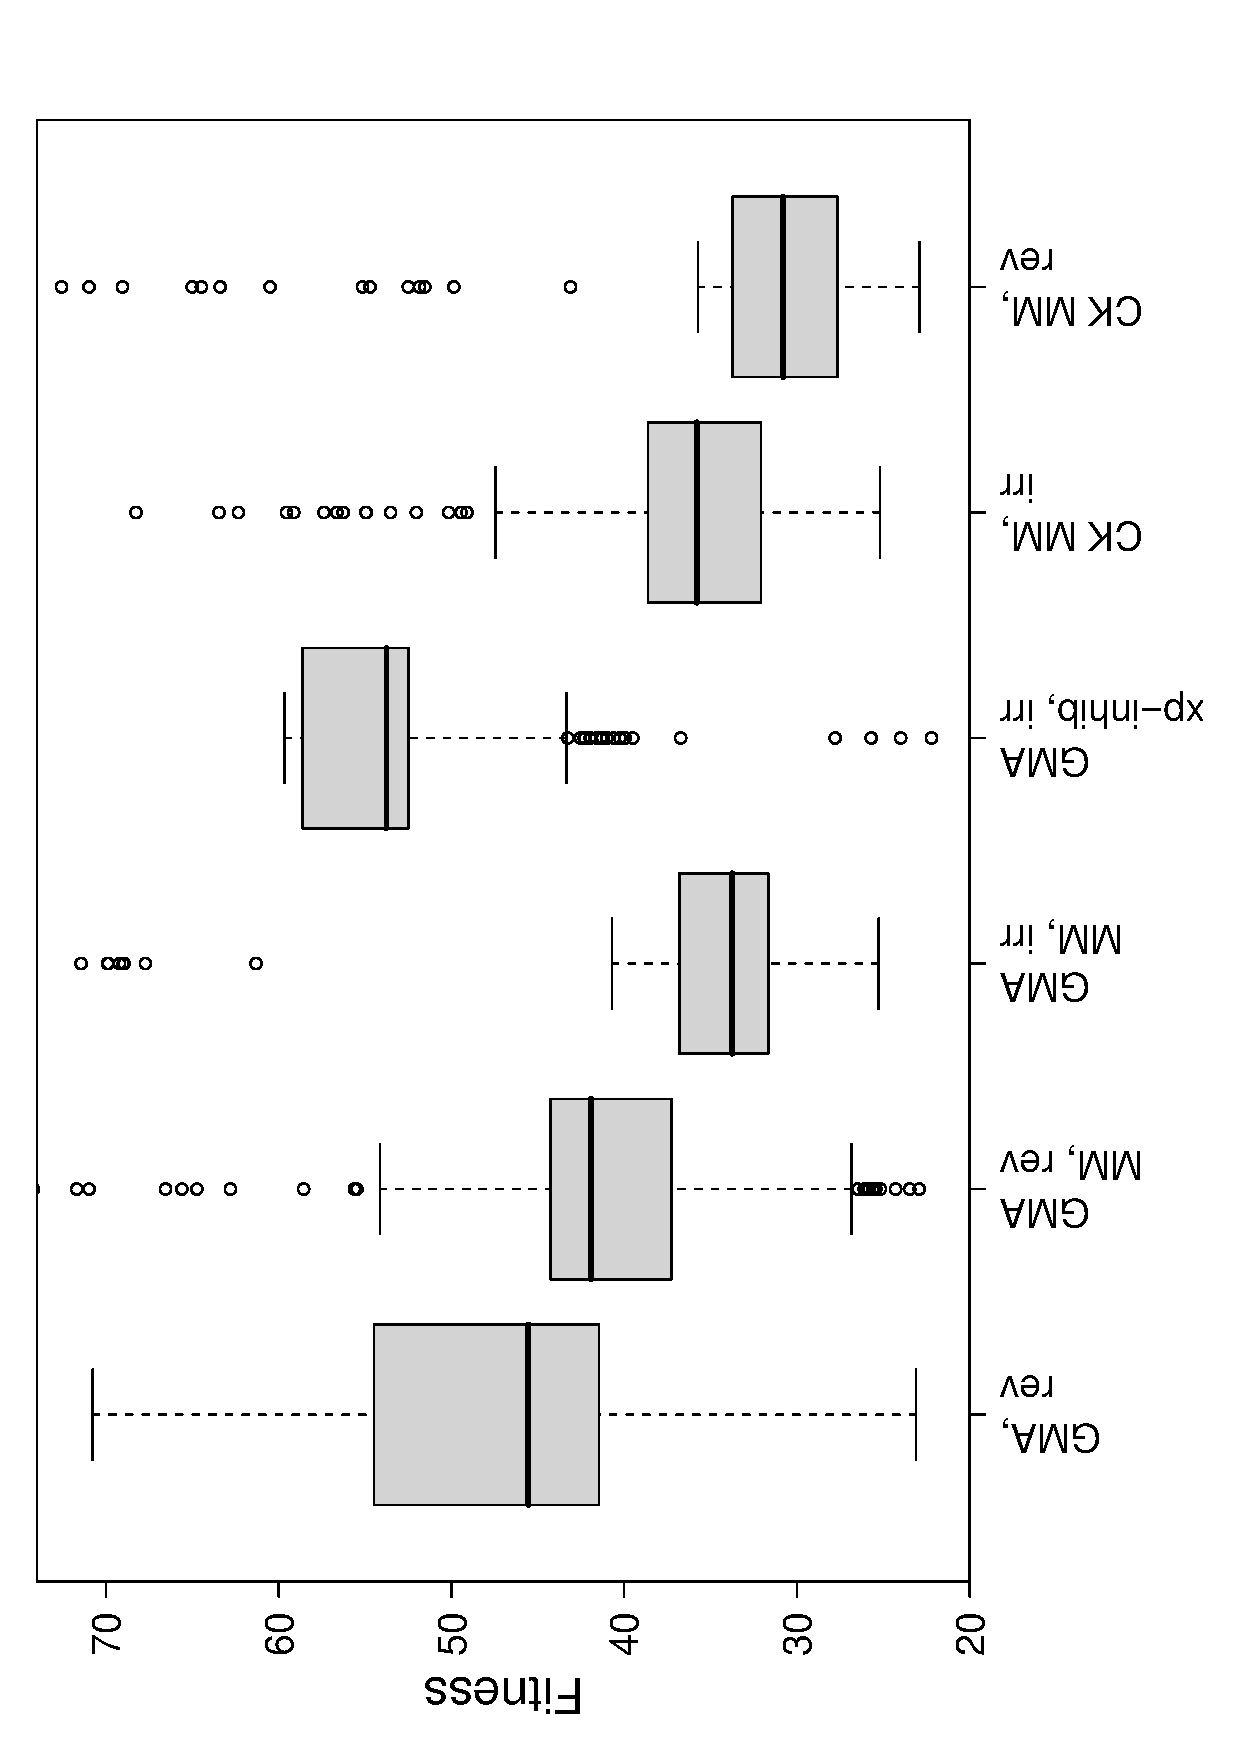
\includegraphics[width=.35\textwidth, angle=90]{img/Modellvergleich}
\label{subfig:ZweitesBild}}}
\caption{Beschriftung für beide Bilder \ref{subfig:ErstesBild} und
\ref{subfig:ZweitesBild}}\label{fig:ZweiBilder}
\begin{small}
Zusätzlicher Text, der die Bilder näher beschreibt, kann hier erfolgen. Bilder
müssen aber nicht mit \verb!\subfigure! gesetzt werden. In vielen Fällen ist die
alleinige Verwendung von \verb!\includegraphics! in Ordnung.
\end{small}
\end{figure}


\subsection{Mathematische Formeln}

Formeln sollen stets mit einer Nummer versehen werden, auch wenn im Text kein
Verweis auf diese Formel erfolgt. Ansonsten kann auch im fließenden Text mit
\verb!$formel$! eine Formel gesetzt werden:
$f_\mathrm{RSE}(\mathbf{\hat x}, \mathbf{X}) =
\sum_{i=1}^{\dim(\mathbf{\hat x})}\sum_{t=1}^T\left(\frac{\hat x_i(\tau_t) -
x_{ti}}{x_{ti}}\right)^2$. Dies ist für größere Formel wie diese aber eher zu
vermeiden.
Falls eine Formel nicht auf eine Zeile passt, kann diese auch auf mehrere Zeilen
aufgeteilt werden, wobei die \verb!eqnarray!-Umgebung vermieden werden sollte:
\begin{align}
v_j =& \frac{k_{+j}^\ce{cat}\prod_i
     \left(\frac{S_i}{K_{ji}^\ce{M}}\right)^{n_{ij}^-} -
     k_{-l}^\ce{cat} \prod_i \left(\frac{S_i}{K_{ji}^\ce{M}}\right)^{n_{ij}^+}}{
     \prod_i\sum_{m=0}^{n_{ij}^-} \left(\frac{S_i}{K_{ji}^\ce{M}}\right)^m +
     \prod_i\sum_{m=0}^{n_{ij}^+} \left(\frac{S_i}{K_{ji}^\ce{M}}\right)^m - 1}
     \nonumber\\
     &\cdot [\ce{E}_j] \cdot \prod_m h_\ce{A}(S_m,K_{jm}^\ce{A})^{w_{jm}^+}
     h_\ce{I}(S_m, K_{jm}^\ce{I})^{w_{jm}^-}
\end{align}
Hier die gleiche Gleichung einmal mit der \verb!multline!-Umgebung:
\begin{multline}
v_j = [\ce{E}_j] \cdot \prod_m h_\ce{A}(S_m,K_{jm}^\ce{A})^{w_{jm}^+}
     h_\ce{I}(S_m, K_{jm}^\ce{I})^{w_{jm}^-}\\
     \cdot\frac{k_{+j}^\ce{cat}\prod_i
     \left(\frac{S_i}{K_{ji}^\ce{M}}\right)^{n_{ij}^-} -
     k_{-l}^\ce{cat} \prod_i \left(\frac{S_i}{K_{ji}^\ce{M}}\right)^{n_{ij}^+}}{
     \prod_i\sum_{m=0}^{n_{ij}^-} \left(\frac{S_i}{K_{ji}^\ce{M}}\right)^m +
     \prod_i\sum_{m=0}^{n_{ij}^+} \left(\frac{S_i}{K_{ji}^\ce{M}}\right)^m - 1}
\end{multline}
Hier wurde die Numerierung der Formel in der ersten Zeile mit dem
\verb!\nonumber!-Befehl unterdrückt.
Wenn Variablen im Fließtext auftreten, müssen diese immer in \verb!$variable$!
eingeschlossen werden, um im Mathematikmodus gesetzt zu werden. Ein Beispiel:
$n$. Bezeichner zu Variablen, die keine Indizes sind, sowie Text in Formel
werden hingegen nicht kursiv gesetzt:
\begin{equation}
 f(x) = \begin{cases}
  \nicefrac{1}{x_\text{kin}^2} & \text{falls }x_\text{kin} \neq 0\\
  0 & \text{sonst}
 \end{cases}
\end{equation}

Abschließend wird in diesem Abschnitt noch ein Beispiel für eine Definition
gegeben:
\begin{definition}[Alphabet]\label{def:Alphabet}
Ein Alphabet $\Sigma $ ist eine nicht leere und beschränkte Menge von Symbolen
mit der Kardinalität $|\Sigma|$. Jedes Alphabet enthält das leere Symbol
$\varepsilon$.
\end{definition}
\begin{satz}
Die Dreiecksungleichung gilt.
\end{satz}
\begin{proof}[Beweis der Dreiecksungleichung]
Ein Beweis.
\end{proof}
\begin{proof}[Widerspruchsbeweis]
\renewcommand{\qedsymbol}{\lightning}
Ein Widerspruchsbeweis.
\end{proof}
\begin{bem}
Eine Anmerkung zu diesem Beweis.
\end{bem}


\subsection{Tabellen}
Ein Beispiel für eine Tabelle über mehrere Seiten ist in
Tabelle~\ref{tab:Pakete} zu sehen. Ein Beispiel für eine Tabelle, die chemische
Formeln enthält, ist durch Tabelle~\ref{tab:Chemie} gegeben. Chemische
Reaktionsgleichungen können mit dem im \verb!styles!-Verzeichnis enthaltenen
\verb!mhchem!-Paket gesetzt werden. Eine Anleitung zu diesem Paket liegt im
selben Verzeichnis.
\begin{table}[htbp]
\begin{center}
\begin{tabular}{llll}
\toprule
Nr.&Reaktion&Enzym&Inhibitor\\
\midrule
$R_1$&\ce{2Pyr -> AcLac + CO2}&\ce{AHAS}&Val\\
$R_2$&\ce{AcLac + NADPH2 <=> DHIV + NADP+}&\ce{AHAIR}&Val\\
$R_3$&\ce{DHIV -> KIV + H2O}&\ce{DHAD}&Val\\
$R_4$&\ce{KIV + Glut -> Val + $\alpha$KG}&\ce{BCAAT_{ValB}}&\\
$R_5$&\ce{KIV + Ala -> Val + Pyr}&\ce{BCAAT_{ValC}}&\\
$R_6$&\ce{Val -> Val_{ext}}&\ce{Trans_{Val}}&Leu\\
$R_7$&\ce{KIV + AcCoA -> IPM + CoA}&\ce{IPMS}&Leu\\
$R_8$&\ce{IPM + NAD+ -> KIC + NADH2 + CO2}&\text{IPMDH}&\\
$R_9$&\ce{KIC + Glut <=> Leu + $\alpha$KG}&\ce{BCAAT_{LeuB}}&\\
$R_{10}$&\ce{Leu -> Leu_{ext}}&\ce{Trans_{Leu}}&Val\\
\bottomrule
\end{tabular}
\end{center}
\caption{Ein System chemischer Reaktionen mit \texttt{booktabs}}
\label{tab:Chemie}
\begin{small}
An dieser Stelle kann eine detailliertere Erklärung zur Tabelle erfolgen.
Wie bei Abbildungen werden Tabellenüberschriften unter die Tabelle gesetzt.
\end{small}
\end{table}
Tabllen sollten möglichst keine vertikalen Trennelemente aufweisen.

\subsection{Darstellung von Algorithmen}
\subsubsection{Pseudocode}
Mit dem \verb!algorithm!-Paket können Algorithmen in einer Gleitumgebung
eingebettet werden. Mit dem \verb!algorithmic!-Paket wiederum können dann
Algorithmen im Pseudocode dargestellt werden (siehe
Algorithmus~\ref{alg:Pseudocode}).
\begin{algorithm}[htbp]
\begin{algorithmic}[1]
\caption{Ein \textit{Hello World}-Programm}
\label{alg:Pseudocode}
\REQUIRE{heutiges Datum $d$}
\ENSURE{"`Hallo Welt"' wird auf den Bildschirm geschrieben}
\FOR{$i \leftarrow 12$ \textbf{downto} $0$}
  \STATE $j \leftarrow 2$
  \COMMENT{Eine Zuweisung}
  \REPEAT
    \IF[Ein Kommentar]{$\nicefrac{i}{j} = 6$}
      \STATE $j \leftarrow 0$
    \ELSIF[Noch ein Kommentar]{$i = 0$}
      \STATE Tu etwas sinnvolles
    \ELSE
      \STATE Warte kurz
    \ENDIF
  \UNTIL{$j = 0$}
\ENDFOR
\STATE print("`Hallo Welt\textvisiblespace"' + $d$)
\STATE \textbf{return true}
\end{algorithmic}
\end{algorithm}

\subsubsection{Auszug aus dem Quellcode}
In einigen Fällen ist es zweckmäßig, ein ganzes Programm einzubinden. Der
Pseudocode ist wegen seiner Kürze jedoch zu bevorzugen. Die
\verb!algorithm!-Umgebung kann auch dazu eingesetzt werden. Für die Darstellung
des Quellcodes muss zur Syntaxhervorhebung dem \verb!listings!-Paket mitgeteilt
werden, um welche Sprache es sich handelt. Anschließend kann die Quelldatei
direkt eingebunden werden (siehe Algorithmus~\ref{alg:Quellcode}).
\begin{algorithm}[htbp]
\caption{Ein einfaches GUI-Programm in Java}\label{alg:Quellcode}
\lstset{language=Java}
\lstinputlisting{src/Visualizer.java}
\end{algorithm}


\subsection{Zitieren}

Ein paar Beipsiele für richtiges Zitieren \cite{Neukam2003}, oder
\cite[Kap.~2]{Neukam2003}.


\section{Die in diesem Dokument enthaltenen Pakete}

Nachfolgend werden alle im WSI-RA-Stil-Dokument eingebundenen Pakete aufgeführt.
\begin{longtable}{p{.2\textwidth}p{.75\textwidth}}
\toprule
\textbf{Paket} & \textbf{Funktion}\\
\midrule
\endfirsthead
\toprule
\textbf{Paket} & \textbf{Funktion}\\
\midrule
\endhead
\multicolumn{2}{c}{Fortsetzung folgt\dots}\\
\endfoot
\endlastfoot
\multicolumn{2}{l}{\bf Grundlegendes für die Sprache}\\
\texttt{ngerman}		& Unsterstützung der aktuellen deutschen Rechtschreibung\\
\texttt{babel}		& Unterstützung mehrsprachiger Dokumente, Spache als Option
angeben. Standardmäßig deaktiviert\\
\texttt{inputenc}	& Erlaubt direkte eingabe aller deutschen Schriftzeichen\\
\multicolumn{2}{l}{\bf Ersetzung der Standard-Schriftarten}\\
\texttt{courier}		& Schreibmaschinen-Schrift\\
\texttt{mathptmx}		& Standardschriftart für den Fließtext\\
\texttt{helvet}	& Standardschriftart für serifenlosen Text\\
\texttt{eurosym}	& Eurosymbol als \euro{} mit dem Befehl \verb!\euro!\\
\multicolumn{2}{l}{\bf Stil}\\
\texttt{geometry}		& Nutzt die A4-Seiten besser aus und setzt den Satzspiegel
neu.\\
\texttt{fancyhdr}		& Gestaltung der Kopf- und Fußzeilen\\
\texttt{bibgerm}	& Deutsche Spracheinstellung für den Zitierstil\\
\texttt{url}		& Schönere Darstellung von Pfadangaben sowie Links ins Web\\
				& bzw. zum E-Mail-Klienten\\
\texttt{hyperref}		& Ermöglicht Links im Dokument, kann aber in einigen Fällen
zu Problemen führen. Das URL-Paket reicht an sich aus. Es wird erst nach der
Überprüfung, ob PDF\LaTeX{} oder \LaTeX{} zum Übersetzen benutzt wird,
eingebunden.\\
\multicolumn{2}{l}{\bf Mathematikpakete}\\
\texttt{nicefrac}		& Schönere Darstellung von Brüchen im Text.\\
\texttt{amsmath}		& Mathematischer Formelsatz mit erweiterten Fähigkeiten\\
\texttt{amsthm}	& \\
\texttt{amscd}	& \\
\texttt{amsfonts}		& Mathematische Schriftarten\\
\texttt{amssymb}		& Mathematik-Symbole\\
\texttt{wasysym}		& Gibt eine Reihe zusätzlicher Symbole, z.\,B.
Widerspruchsblitz.\\
\multicolumn{2}{l}{\bf Chemiepaket}\\
\texttt{mhchem}
				& Erlaubt chemische Formeln\\
\multicolumn{2}{l}{\bf Notwendige Pakete für Grafiken und Farbe}\\
\texttt{graphicx}		& Einbinden von Grafik-Dateien\\
\texttt{epsfig}		& Einbinden von EPS-Graphiken. Nur aktiviert, wenn
PDF\LaTeX{} benutzt wird.\\
\texttt{psfig}		& Einbinden von PS-Graphiken. Nur aktiviert, wenn
PDF\LaTeX{} benutzt wird.\\
\texttt{subfigure}		& Unterabildungen in figure-Umgebungen\\
\texttt{color}		& Farbiger Text ermöglicht. Standardmäßig deaktiviert\\
\multicolumn{2}{l}{\bf Für Tabellen}\\
\texttt{longtable}		& Unterstützt lange Tabellen, die über mehrere Seiten
gehen.\\
\texttt{multirow}		& Stellt den Befehl für Zellen über mehrere Zeilen zur
Verfügung.\\
\texttt{array}		& Enthält zusätzliche Befehle für komplexe Tabellen\\
\texttt{booktabs}		& Produziert besonders schöne Tabellen.\\
\texttt{dcolumn}		& Ermöglicht nach Dezimalstellen formatierte
Tabelleneinträge. Standardmäßig deaktiviert\\
\texttt{hhline}		& Erweiterte Möglichkeiten für Linien in Tabellen.\\
\multicolumn{2}{l}{\bf Algorithmuspakete}\\
\texttt{algorithm}	& Stellt eine Gleitumgebung für Algorithmen zur Verfügung.\\
\texttt{algorithmic}    & Ermöglicht Einbindung von Algorithmen im Pseudo-Code,
die dann auch ins Algorithmenverzeichnis aufgenommen werden.\\
\texttt{listings}		& Quellcode einbinden. Mit \lstset{language=C++} o. Ä. wie
C, C++, Java, VHDL, Ada, Fortran, HTML, Mathematica, Pascal, Perl, Python\dots
Sprache wählen und mit
\verb!\lstinputlisting{meine-datei.cpp}! einfach einbinden.\\
\multicolumn{2}{l}{\bf Für Tabellen oder Abbildungen, die eine Seite im
Querformat beanspruchen}\\
\texttt{lscape}		& Funktioniert nur mit dem herkömmlichen \verb!latex!.\\
\texttt{pdflscape}	& Funktioniert nur mit \verb!pdflatex!.\\
\multicolumn{2}{l}{\bf Abkürzungsverzeichnis, Glossar und Index}\\
\texttt{abbrev}		& Bietet ein Abkürzungsverzeichnis\\
\texttt{makeidx}		& Ermöglicht Erstellung eines Indexes.
Standardmäßig deaktiviert\\
\texttt{glossary} & Erlaubt die Erstellung eines Glossars.\\
\bottomrule
\caption{Die in diesem Dokument geladenen \LaTeX-Pakete}\label{tab:Pakete}
\end{longtable}


\section{Anmerkungen zu den Literaturverweisen}
\label{sec:HinweiseLiteratur}

Eine Hilfe zum richtigen Zitieren und Schreiben des Literaturverzeichnisses
bietet \textsc{Bib}\-\TeX, das auf der Webseite
\url{http://de.wikipedia.org/wiki/BibTeX} ausf"uhrlich erkl"art wird.
Dabei ist zu beachten, dass je nach der Art des zu zitierenden Werkes spezielle
Einträge in der \textsc{Bib}\TeX-Datei geben kann. Tabelle~\ref{tab:bibTeX} gibt
eine Übersicht über die wichtigsten Arten von Quellen und die von
\textsc{Bib}\TeX vorgesehenen Einträge für das Literaturverzeichnis. Eine Hilfe
zum Erstellen und Verwalten von Literaturreferenzen bietet das Programm
\textsc{JabRef} (\url{http://jabref.sourceforge.net},
Abbildung~\ref{fig:JabRef}). Dieses in Java implementierte und dadurch
plattformunabhängige Programm bietet eine leicht verständliche und
übersichtliche graphische Nutzeroberfläche, die u.\,a. eine Suchfunktion
enthält, sodass auch nach Stichwörtern in Publikationen gesucht werden kann.
Des Weiteren lassen sich damit auch die zugehörigen PDF-Dateien
verwalten.
\begin{figure}[htbp]
 {\centering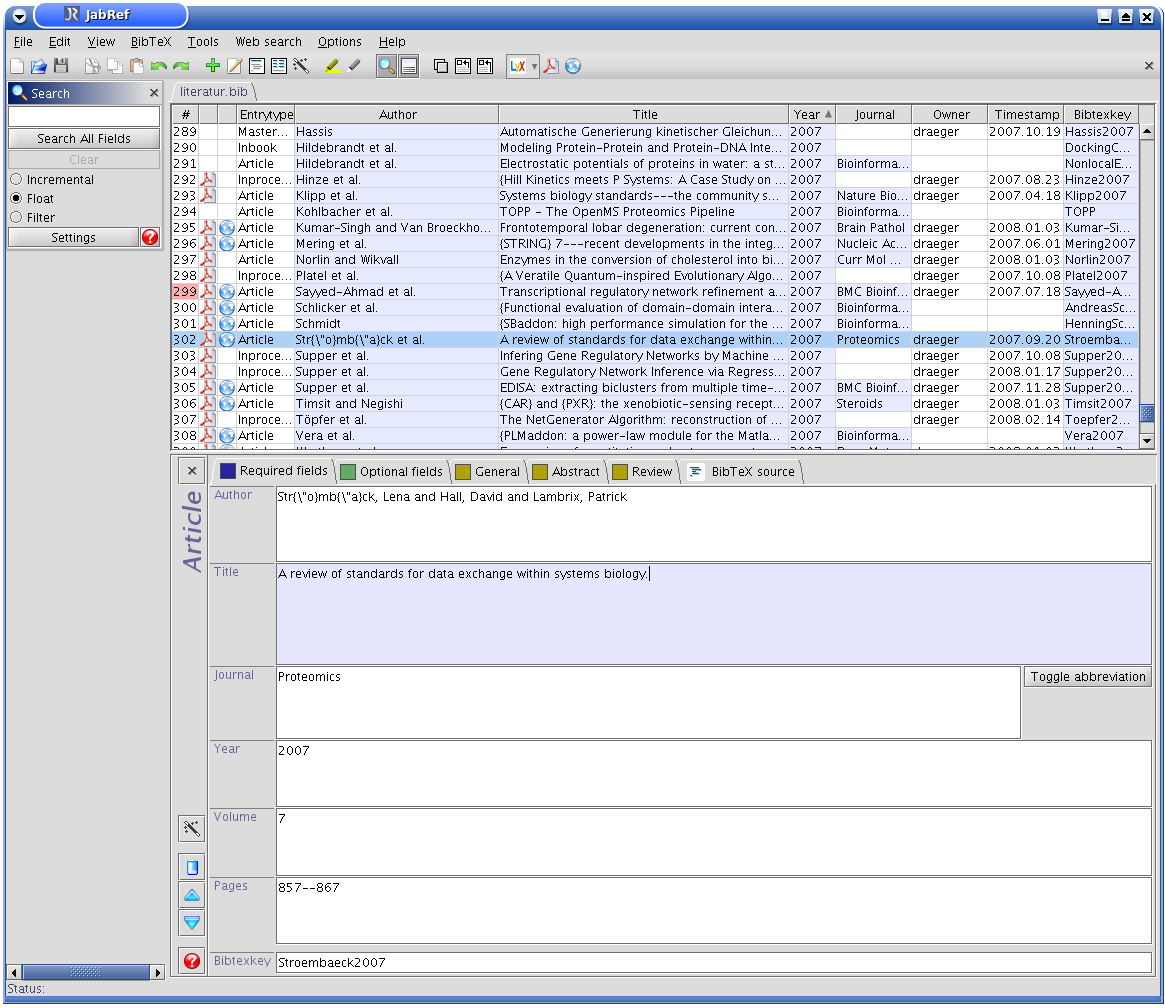
\includegraphics[width=\textwidth]{img/jabref}
 \caption{Der Referenzmanager \textsc{JabRef}}\label{fig:JabRef}}
 \begin{small}
 Die Suchfunktion erlaub eine Stichwortsuche in der gesamten Literaturliste.
 Mit einem Rechtsklick, hier auf "`Article"', kann auch die Art der
 Veröffentlichung geändert werden, wobei sich automatisch die Liste der
 vorzunehmenden einträge anpasst. Importfunktionen ermöglichen, z.\,B.
 XML-Dateien direkt von PubMed in die Literaturliste einzufügen, ohne dass alle
 Informationen abgetippt werden müssen.
 \end{small}
\end{figure}
\begin{table}[htbp]
\centering
\begin{tabular}{p{.2\textwidth}p{.35\textwidth}p{.35\textwidth}}
\toprule
Referenzart & notwendige Felder & optionale Felder\\
\midrule
article & author, title, journal, year & volume, number, pages, month, note\\
book & author or editor, title, publisher, year & volume or number, series,
address, edition, month, note, isbn\\
booklet & title & author, howpublished, address, month, year, note\\
conference & author, title, booktitle, year & editor, volume or number, series,
pages, address, month, organization, publisher, note\\
inbook & author or editor, title, chapter and/or pages, publisher, year & volume
or number, series, type, address, edition, month, note\\
incollection & author, title, booktitle, publisher, year & editor, volume or
number, series, type, chapter, pages, address, edition, month, note\\
inproceedings & author, title, booktitle, year & editor, volume or number,
series, pages, address, month, organization, publisher, note\\
manual & title & author, organization, address, edition, month, year, note\\
mastersthesis & author, title, school, year & type, address, month, note\\
misc & - & author, title, howpublished, month, year, note\\
phdthesis & author, title, school, year & type, address, month, note\\
proceedings & title, year & editor, volume or number, series, address, month,
organization, publisher, note\\
techreport & author, title, institution, year & type, number, address, month,
note\\
unpublished & author, title, note & month, year\\
\bottomrule
\end{tabular}
\caption{Literaturtypen}
\label{tab:bibTeX}
\end{table}

Eine grundlegende Einführung in \LaTeXe{} ist in \cite{Schmidt2003} gegeben.
Diese eignet sich, um einen schnellen Einstieg und Überblick über die meisten
Funktionen zu erhalten. In \cite{Juergens2000} bekommt der Leser ebenfalls einen
guten Einstieg in \LaTeX. Der zweite Band dieses Werkes \cite{Juergens1995} gibt
Überblick über viele interessante Funktionen, die zusätzlich das Interesse an
diesem Satzsystem erhöhen.

Die Feinheiten des \KOMAScript-Paketes, dessen \verb!scrreprt!-Stil diesem
Dokument zu Grunde liegt, werden in \cite{Neukam2003} ausführlich behandelt.

Was beim Schreiben mit der Maschine zu beachten ist, und wie die Regeln des
Dudens und des DINs speziell in \LaTeX{} umgesetzt werden können, ist
\cite{Struckmann2004} zu entnehmen. Wie wissenschaftliche Texte mit \LaTeX{}
verfasst werden können, wird ausführlich in \cite{Farwer2005} behandelt.

% \input{tex/02_Methoden}
% \input{tex/03_Ergebnisse}
% \input{tex/04_Diskussion}
% \input{tex/05_Schlussfolgerungen}
% \input{tex/06_ZsfundAusblick}


%%%%%%%%%%%%%%%%%%%%%%%%%%%%%%%%%
% Der Anhang                    %
%%%%%%%%%%%%%%%%%%%%%%%%%%%%%%%%%

\appendix
\begin{abbreviations}
   \abbrev*{trna}{tRNA}{Transfer-RNA}
%   \abbrev*{api}{\mbox{API}}{\it Application Programming Interface}
 % \abbrev*{awt}{\mbox{AWT}}{\it Abstract Windowing Toolkit}
 %  \abbrev*{blast}{\mbox{BLAST}}{\it Basic Local Alignment Search Tool}
 % \abbrev*{cvs}{\mbox{CVS}}{\it Concurrent Version System}
\end{abbreviations}

% Erzeuge Glossar und Index.
% Aufruf: makeindex -t Vorlage.glg -o Vorlage.gls -s Vorlage.ist
% Vorlage.glo
% \glossary{name={Ortholog},description={Homologe Proteine oder Gene in
% verschiedenen Organismen, die sich von einem gemeinsamen Vorläufergen durch
% Spezialisierung entwickelt haben. Normaler Weise behalten Orthologe die gleiche
% Funktion im Verlauf der Evolution.}}
%
% \glossary{name={Paralog},description={Homologe Proteine oder Gene, die im
% gleichen Organismus verschiedene Funktionen ausüben und meist durch Duplikation
% innerhalb eines Genoms entstanden sind. Im Gegensatz zu Orthologen entwickeln
% Paraloge neue Funktionen, selbst wenn diese den originalen Funktionen ähneln.}}
%
% \glossary{name={Homolog},description={Ein Gen oder Protein, das mit einem anderen Gen oder 
% Protein verwandt ist, da beide von einer gemeinsamen Vorgänger-DNA-Sequenz abstammen. Der 
% Term \frqq homolog\flqq\ kann zur Beziehung zwischen Genen \mbox{bzw.}~Proteinen verwendet 
% werden, die durch eine Spezialisierung (\mbox{vgl.}~ortholog) oder durch das Ereignis der 
% Genduplikation (\mbox{vgl.}~paralog) entstanden sind.}}

% Aufruf: makeindex -t Vorlage.glg -o Vorlage.gls -s Vorlage.ist Vorlage.glo
\printglossary
% \printindex

%%%%%%%%%%%%%%%%%%%%%%%%%%%%%%%%%
% Das Literaturverzeichnis      %
%%%%%%%%%%%%%%%%%%%%%%%%%%%%%%%%%

% Dadurch werden die Zitate mit abgekürzten Namen der Autoren generiert.
\bibliographystyle{ra-alpha}
\bibliography{tex/Literatur}

\end{document}
